%!TEX root = ../csuthesis_main.tex

\section{相关理论基础}
本章围绕音频分类任务，介绍量子时序编码和量子时频分析神经网络涉及的理论基础。当前人工智能与量子计算相互结合，催生了量子机器学习，这给突破传统深度学习算力和存储瓶颈提供了一种可能。本节先从量子比特、逻辑门、叠加纠缠特性以及测量原理入手，梳理量子计算的物理和数学基础\citess{nielsen2010quantum}。量子计算用量子比特取代了经典比特，依靠它特有的叠加和纠缠性质，解决复杂模式识别问题有了提速的希望。接着，本研究讨论了量子特征映射理论，在对比几种常见量子编码方式后，重点分析了增强型量子表示（NEQR）技术，这就为后续把经典音频特征转成量子态提供了理论依据。最后，本节剖析了量子神经网络（QNN）的架构和运行机制，包括状态编码器、参数化量子线路以及测量模块，并探讨了如何在含噪中等规模量子（NISQ）设备上对其进行优化。这些内容构成了本文构建量子时频分析模型的底层依据。
\subsection{量子计算基础}
量子计算是一门横跨计算机科学、量子力学、线性代数和信息论的交叉学科。它借用量子力学的基本假设，能在高维希尔伯特空间里并行处理信息，这就给经典计算机在算大规模复杂张量时遇到的瓶颈提供了一条解决途径\citess{10.1109/TPAMI.2022.3203157}。特别是在碰到特征维度极高且依赖长序列的场景时，量子计算在存储和运算上的优势更加明显。本节将具体介绍它的核心原理。

\subsubsection{量子比特与逻辑门}
经典计算里，信息一般用经典比特表示，物理状态是确定的，要么是 0 要么是 1。量子计算则不同，它把量子比特当作存数据和处理数据的基本单元\citess{Rezaul2024}。量子比特其实是二维复希尔伯特空间里的一个向量，它不但能表示基态 $\ket{0}$ 和 $\ket{1}$，还能按任意复数比例同时处于这两个状态的叠加之中。用狄拉克符号写出来为：
\begin{equation}
	\ket{\psi} = \alpha\ket{0} + \beta\ket{1} 
\end{equation}

这里的 $\alpha$ 和 $\beta$ 是复数形式的概率幅，代表系统被观测后坍缩成 $\ket{0}$ 和 $\ket{1}$ 的幅度。根据玻恩法则，这两个系数模长的平方和必须等于 1，也就是 $|\alpha|^2 + |\beta|^2 = 1$。受这个特性影响，$n$ 个量子比特组成的系统能同时处于 $2^n$ 种状态的叠加中。所以量子计算机做一次操作，就能并行处理呈指数级增长的信息，从而在本质上大幅提高了处理效率\citess{shi2024qsan,zhao2024qksan, arute2019quantum}。

在量子线路里，量子门负责执行基础逻辑操作。它们主要通过对量子比特的态矢量做线性代数变换，来完成信息的演化。如果量子系统是封闭的，那它的状态演化就是完全可逆的，可以用一个酉矩阵 $U$ 来严谨描述\citess{shi2024pretrained}。在数学上，酉矩阵必须满足 $UU^{\dagger}=I$（其中 $U^{\dagger}$ 是 $U$ 的共轭转置\citess{yu2023optimal}）。

为了构建复杂的量子算法，通常需要组合多种基础量子门。常见的单比特量子门包括：用于生成均匀叠加态的 Hadamard 门（H门）\citess{peral2024systematic,garcia2024mitigating}、用于在布洛赫球上绕 X 轴旋转 $\pi$ 角度从而翻转量子态的 Pauli-X 门，以及用于相位调整的 Pauli-Z 门和各种旋转门（如 $R_x, R_y, R_z$）\citess{ropa2021introduction}。在多比特操作中，控制非门（CNOT门）是实现量子纠缠不可或缺的关键组件\citess{peral2024systematic}。主要基础量子门及其对应的矩阵表示如表 \ref{tab:quantum_gates} 所示：


\begin{table}[htb]
	\caption{常见基础量子门及其矩阵表示}
	\label{tab:quantum_gates}
	\centering
	\begin{tabular}{ m{2cm}<{\centering} m{3cm}<{\centering} m{3cm}<{\centering} }
		\toprule
		量子门名称 & 电路图表示 & 矩阵表示 \\
		\midrule
		单位门 ($I$) & \begin{minipage}{0.3\columnwidth}\Qcircuit @C=1em @R=1em {&\gate{I} & \qw }\end{minipage} & $\begin{pmatrix} 1 & 0 \\0 & 1 \end{pmatrix}$ \\
		Hadamard门 ($H$) & \begin{minipage}{0.3\columnwidth}\Qcircuit @C=1em @R=1em {&\gate{H} & 
				\qw }\end{minipage} 
		& $\begin{pmatrix} \frac{\sqrt{2}}{2} & \frac{\sqrt{2}}{2} \\ \frac{\sqrt{2}}{2} & -\frac{\sqrt{2}}{2} \end{pmatrix}$ \\
		Pauli-X门 ($X$) & \begin{minipage}{0.3\columnwidth}\Qcircuit @C=1em @R=1em {&\gate{X} & \qw }\end{minipage} & $\begin{pmatrix} 0 & 1 \\1 & 0 \end{pmatrix}$ \\
		控制非门 ($CNOT$) & \begin{minipage}{0.3\columnwidth}\Qcircuit @C=1em @R=1em {& \ctrl{0} \qwx[1] & \qw \\& \targ & \qw }\end{minipage} & $\begin{pmatrix} 1 & 0 & 0 & 0 \\0 & 1 & 0 & 0\\0 & 0 & 0 & 1\\0 & 0 & 1 & 0\\ \end{pmatrix}$ \\
		\bottomrule
	\end{tabular}
\end{table}


\subsubsection{量子叠加与纠缠特性}
量子计算之所以有强大的并行能力，物理根基就在于量子叠加。经典计算机在做含 $N$ 个可能性的搜索任务时，时间复杂度通常是 $O(N)$；但量子叠加允许计算过程在希尔伯特空间的所有基态上同时演化，这就给 Grover 算法等指数级或多项式级的加速算法创造了条件。

另外，量子纠缠是复合量子系统里特有的一种非局域关联，没法用经典物理学来解释。当几个量子比特纠缠在一起时，整个系统的量子态就没法再拆解成各个独立状态的张量积了\citess{tao2024quantum}。换句话说，只要测了其中一个粒子，另一个粒子的状态瞬间就确定了，并且这种强关联完全不受它们物理距离的影响。

在设计量子线路时，通常是把受控门（比如 CNOT 门或 iSWAP 门）作用在已经是叠加态的量子比特上，以此来制备纠缠态。贝尔态是最有代表性的最大纠缠态\citess{mishra2024transformation}，它四个正交基里的其中一个，数学表达式如下：
\begin{equation}
	\ket{\Phi^{+}} = \frac{1}{\sqrt{2}} (\ket{00} + \ket{11})
\end{equation}
挖掘数据特征时，非经典纠缠可视作核心计算资源。网络系统借此捕获高维空间的非线性映射关系。面对音频等多维时间序列，现有方法常利用量子纠缠机制建立长跨度全局上下文依赖，并深度绑定局部时间步特征。
\subsubsection{量子测量原理}
尽管量子系统在其演化过程中处于高度复杂的叠加状态，但当我们试图获取最终的计算结果时，量子测量起着不可逆的决定性作用。由于量子比特在未被观测时处于不确定的概率叠加态，必须通过物理测量操作使其坍缩到一个确定的经典状态，从而提取出有效的计算结果。

在量子力学的标准框架下，测量通常由一组正交投影算符或正定算子值测量来定义。测量过程会将系统不可见的量子态投影到一种可观测的基态上，将其转化为经典的实值数据（0或1）以供后续分析。需要指出的是，单次量子测量具有随机性，其得到特定结果的概率由量子态在该基矢上的概率幅模长平方决定。

在实际应用于分类任务的量子神经网络模型中，通常会固定选取网络末端的若干个输出量子比特，执行基于 Pauli-Z 算符的测量。假设量子系统在测量前处于最终演化态 $\ket{\varphi}$，为了消除单次测量的随机性并获得平滑的输出以供计算损失函数（如二元交叉熵损失），通常需要对同一量子线路进行多次重复采样（Shots），以此来逼近该算符的统计期望值：
\begin{equation}
	E 
	= \bra{\varphi} Z \ket{\varphi}
\end{equation}
通过上述测量机制，量子模型成功地将高维希尔伯特空间中的复杂量子演化数据转换为与经典深度学习框架相兼容的实数输出形式，完成了从量子特征空间到经典概率分布的最终映射。

\subsection{量子特征映射理论}
在经典与量子混合计算架构下，底层量子硬件无法直接处理音频 MFCC 矩阵等经典张量。因此，必须引入状态编码器将经典数据转换并写入量子态，此过程即为量子特征映射\citess{schuld2019quantum, havlivcek2019supervised}。特征映射方案的选择直接决定了模型所需的量子比特数（空间复杂度）与线路深度（时间复杂度），并对后续网络的特征表征精度及分类性能产生实质性影响。

\subsubsection{常见量子编码方式}
数据编码是将经典特征导入量子网络的前置环节。结合数据规模、维度特征与硬件约束，学术界目前主要采用以下三种基础编码技术\citess{ranga2024quantum}：

（1）基态编码：该方法通过直接映射逻辑，将经典二进制串或离散整型转换为对应的量子计算基态。例如，数值 $x = 5$（二进制 101）被映射为 $\ket{101}$。其规则较为直观，但量子比特的消耗量与数据位宽呈严格线性正相关，在处理高维连续特征时容易遭遇硬件资源瓶颈。

（2）振幅编码：此方法通过调控量子态基矢的振幅来连续表示特征向量\citess{ranga2024quantum}。对于 $N$ 维输入向量 $\vec{x} = (x_1, x_2, \dots, x_N)$，在满足 $\sum |x_i|^2 = 1$ 的物理约束下，可转化为：
\begin{equation}
	\ket{\psi} = \sum_{i=1}^{N} x_i \ket{i}
\end{equation}
振幅编码具备较高的信息压缩比，表示 $N$ 维特征仅需 $\log_2 N$ 个量子比特。但在物理制备任意振幅状态时，线路深度的指数级扩张易导致系统受到退相干噪声的干扰，降低了当前硬件条件下的实现稳定性。

（3）角度编码：该方案调用单比特旋转门（如 $R_x(\theta), R_y(\theta), R_z(\theta)$），将连续特征映射为量子态的相位或旋转角度。设输入特征为 $x_i$，通过执行 $\bigotimes R_y(x_i)\ket{0}$ 即可完成独立参数的赋值。凭借 $O(1)$ 的浅层线路深度，该机制在 NISQ 设备端表现出较强的抗噪鲁棒性。

然而，上述常规编码路径通常预设输入特征呈独立且静态的分布。在处理非平稳的音频时序数据时，此类方法难以有效保留全局时间顺序与动态上下文关联，这在客观上推动了具有时间依赖感知能力的量子表示体系的发展。

\subsubsection{增强型量子表示}
增强型量子表示（Novel Enhanced Quantum Representation, NEQR）\citess{zhang2013neqr} 早期多见于数字图像处理领域。该模型旨在缓解灵活量子图像表示模型（FRQI）对振幅精度的过度依赖。NEQR 摒弃了将像素灰度直接耦合至连续振幅的思路，转而引入多量子比特序列的基态来映射离散数值\citess{dong2022novel,chen2022qirhsi,werner2023data}。

NEQR 的底层架构依赖两组相互纠缠的量子比特序列：一组用于绑定像素的色彩或灰度信息；另一组则映射对应的二维空间位置坐标。将这两组序列置入全局叠加态后，可实现整幅图像数据的单量子态加载。其数学表达为：
\begin{equation}
	\ket{I} = \frac{1}{2^n} \sum_{i=0}^{2^{2 n}-1}\ket{c_i} \otimes\ket{i} 
\end{equation}
式中，状态序列 $\ket{c_i} = \ket{c_i^{q-1} \cdots c_i^1 c_i^0}$ 由 $q$ 个量子比特构成，用于记录第 $i$ 个像素的灰度二进制值；坐标序列 $\ket{i} = \ket{y_{n-1}\dots y_0}\ket{x_{n-1}\dots x_0}$ 涵盖横轴与纵轴坐标，负责对 $2^n \times 2^n$ 尺寸图像的空间边界进行位置标定\citess{shi2022image}。

这种基于基态纠缠的编码范式将图像内容与位置上下文整合于单一物理叠加态内。相较于常规振幅编码，NEQR 规避了深层演化线路引发的精度衰减问题，并在量子域图像几何变换操作上提供了计算接口。

在逻辑推导上，NEQR 中“内容与坐标深度耦合”的机制，为高维量子时序数据处理提供了理论参照。若将二维空间坐标等效映射为音频信号的“时间戳”，灰度值等价替代为特定时间帧的“声学特征值（如MFCC）”，该理论范式即可有效迁移。本文后续章节提出的量子时序编码方法即建立在这一逻辑推演之上。

\subsection{量子神经网络}
量子神经网络（Quantum Neural Network, QNN）结合了量子计算理论与经典神经网络的层级拓扑\citess{li2024qea,qu2023qnmf, benedetti2019parameterized}。与传统深度神经网络不同，QNN 的推演过程直接建立在高维希尔伯特空间内，主要依托量子态的叠加并行演化及多粒子纠缠机制来提取高阶特征。相关对比研究显示，在处理同阶复杂度的分类任务时，QNN 系统占用的可训练参数规模通常呈数量级减少，并在特定数据集上表现出优异的泛化能力与抗过拟合特性。

从基础结构拓扑来看，如图 \ref{QNN_structure} 所示，常规的端到端变分 QNN 框架依数据流向可划分为三个核心处理组件\citess{shi2025quantest,gong2024quantum}：

\begin{figure}[!htb]
	\centering
	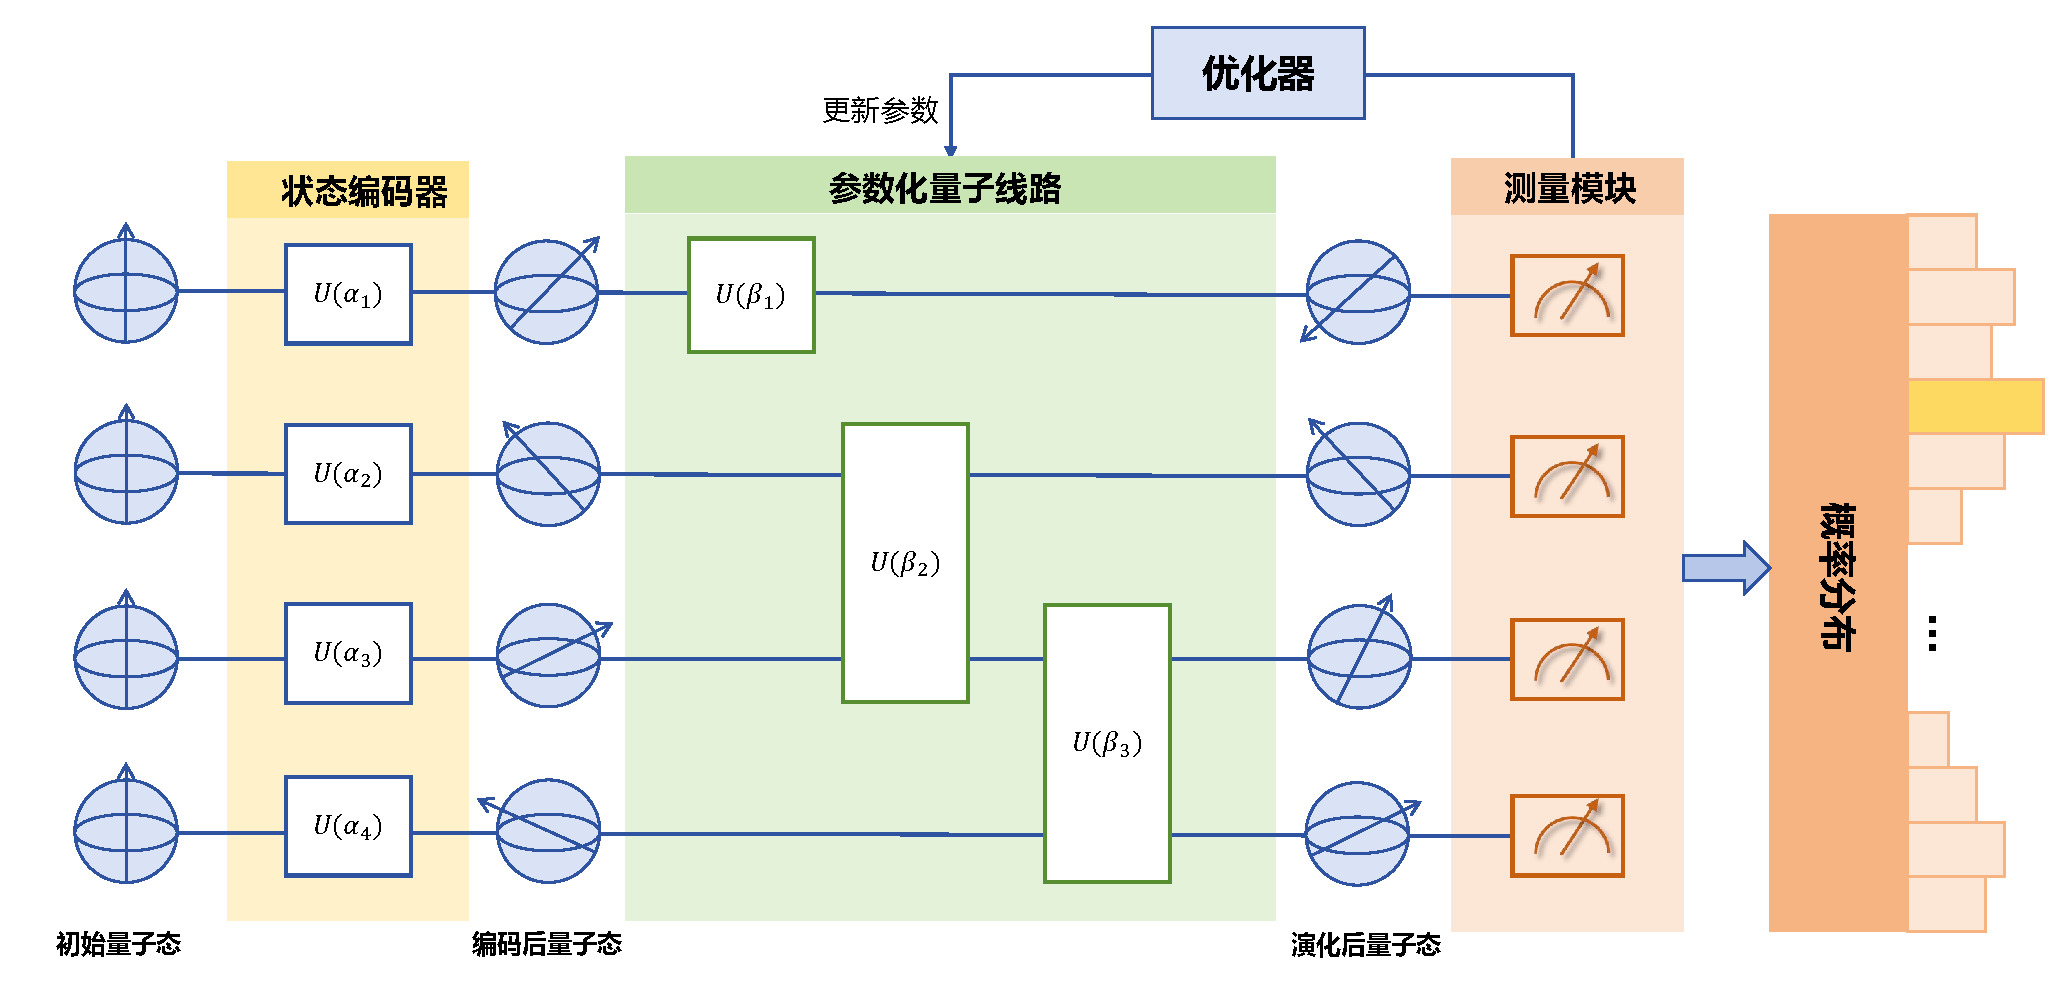
\includegraphics[width=0.8\textwidth]{./images/The structure of QNN.pdf}
	\caption{量子神经网络的基本结构框架}
	\label{QNN_structure}
\end{figure}

（1）状态编码器。该组件在 QNN 框架中承担对标经典网络输入层的数据载入功能。受限于量子硬件的底层读取逻辑，量子芯片及模拟器无法直接接收经典的实数张量数据。因此，编码器需利用预设的映射规则 $S(x)$，将降维后的经典特征向量 $x$转化为初始量子态 $\ket{\psi_{in}} = S(x)\ket{0}^{\otimes n}$。该机制打通了经典数据源与量子逻辑门的操作接口，是后续高维特征提取的必要前置环节。

（2）参数化量子线路（PQC）。作为 QNN 的推理核心模块，PQC 在结构功能上对标经典网络中的隐藏层，负责执行特征提取与高维空间非线性变换\citess{peral2024systematic,huang2024quantum, henderson2020quanvolutional}。为兼顾模型表达精度与物理设备的可执行性，PQC 通常采用硬件高效拟设（Hardware-efficient Ansatz）。从数学角度描述，一个深度为 $L$ 的 PQC 可表示为一系列可调幺正算符与固定纠缠算符的级联乘积：
\begin{equation}
U(\vec{\theta}) = \prod_{l=1}^{L} \left( W_l U_l(\theta_l) \right)
\end{equation}
其内部拓扑由两类逻辑门交替构成：其一为含参单比特旋转门（如 $R_x, R_y, R_z$），用于在布洛赫球域内执行三维相位调制，为网络引入必要的权重分布；其二为无参双比特受控门（如 CNOT 门），负责在量子比特间建立物理纠缠，协助网络提取跨时间步的时序相关性。在训练过程中，核心优化目标是不断更新旋转门的参数向量 $\vec{\theta}$，使得 PQC 最终逼近当前任务下的最优酉变换矩阵。

（3）测量模块。作为 QNN 的输出层，该模块主要负责处理演化后的量子终态 $\ket{\psi_{out}} = U(\vec{\theta})\ket{\psi_{in}}$。通过物理坍缩机制，该模块将高维量子态降维投影为经典计算机可解析的数据。通常系统会计算指定末端量子比特在 Pauli-Z 算符下的期望值：
\begin{equation}
f(x, \vec{\theta}) = \bra{\psi_{out}} \sigma_z \ket{\psi_{out}}
\end{equation}
所获取的期望值序列随后传入经典激活函数或外接的全连接层进行概率归一化，最终映射出分类任务所需的交叉熵损失。

对比经典卷积与循环网络架构，QNN 呈现出特定的计算与优化特征。一方面，网络所需的训练参数量明显减少\citess{tasnim2024comparison,feng2025variational}，这在一定程度上降低了特征提取对大规模数据集的依赖，同时也符合当前 NISQ 设备浅层线路的物理约束。另一方面，在参数寻优环节，QNN 引入了参数平移规则来获取精确的解析梯度：
\begin{equation}
\frac{\partial f(x, \vec{\theta})}{\partial \theta_i} = \frac{f(x, \theta_i + \frac{\pi}{2}) - f(x, \theta_i - \frac{\pi}{2})}{2}
\end{equation}
这一算子机制规避了经典网络中繁杂的链式法则，使量子模型具备了较好的收敛效率\citess{song2024resource, cerezo2021variational}。综合来看，这种将高维量子态演化与经典参数寻优相结合的混合计算范式，在理论上有效平衡了模型的特征表征能力与当前含噪设备的物理约束，为探索资源受限下的复杂感知任务提供了切实可行的基础框架。

\subsection{知识蒸馏}
深度学习模型结构的规模化扩张导致参数量与计算开销剧增，客观上制约了大型网络在资源受限边缘端的部署。为平衡分类性能与硬件资源消耗，模型压缩技术得到广泛应用。其中，知识蒸馏作为一类主流的知识迁移范式，提供了相对有效的压缩路径\citess{yim2017gift}。本节梳理知识蒸馏的底层机制，涵盖教师-学生架构、软标签及温度调控参数、联合损失函数构造，并探讨其向经典-量子跨计算范式迁移的可行性。

\subsubsection{知识蒸馏核心机制}
知识蒸馏机制的雏形最早可追溯至 Buciluǎ 等于 2006 年提出的模型压缩思想\citess{bucilua2006model}，随后 Hinton 等人在 2015 年对其进行了系统化定义，并正式确立了非对称的“教师-学生”网络拓扑作为其核心框架\citess{hinton2015distilling, gou2021knowledge}。该范式打破了传统的物理维度的参数裁剪逻辑，转而关注模型决策行为与内在表征的软性迁移。

在此架构中，教师模型通常是参数庞大、拓扑复杂且经过海量数据充分预训练的高性能网络，具备极高的假设空间，能从复杂信号中学习到高度泛化的深层抽象表征；而学生模型则受限于部署场景的算力约束，表现为结构轻量的微型网络。若独立优化此类轻量模型，受限于网络容量，极易欠拟合或陷入局部极小值。知识蒸馏的核心动机，即引入教师输出作为监督信号，引导学生模型在有限参数下逼近大型网络的泛化边界。

Hinton 的研究深刻揭示了这一性能飞跃的理论基础：传统监督学习依赖“独热（One-hot）”形式的硬标签（Hard Labels），虽明确真实类别，却将非目标类概率置零，抹杀了类别间的拓扑相似度。事实上，高性能分类器输出的概率分布中，非目标类的微小波动蕴含丰富结构化信息。例如在音频识别中，“风声”被误判为“海浪声”的概率理应远高于“警笛声”。此类隐藏在连续概率分布中的跨类别相关性映射，被定义为“暗知识（Dark Knowledge）”\citess{hinton2015distilling}。

为了有效提取并传递暗知识，知识蒸馏在 Softmax 激活阶段引入了带温度缩放的参数 $T$。设定输出端提取的未归一化逻辑值（Logits）为 $z_i$，经参数 $T$ 调控的软概率分布 $p_i$ 表达式如下：
\begin{equation}
	p_i = \frac{\exp(z_i / T)}{\sum_j \exp(z_j / T)}
\end{equation}
当 $T=1$ 时，计算逻辑等同于标准 Softmax 分布。提升 $T$ 的取值可诱导分布趋于平滑，即生成软标签（Soft Labels）。在此状态下，原先接近于 0 的非目标类概率权重得以提升，从而显现出教师模型捕获的类别相似性特征，使暗知识显性化。若 $T \to \infty$，各类别概率将趋于一致，分布向均匀分布退化。通过调节 $T$ 的取值，可实现对暗知识提取尺度的灵活控制。

知识蒸馏的训练过程通常采用硬损失与软损失相加的联合损失函数 $L_{Total}$。其中，硬损失 $L_{hard}$ 衡量标准温度（$T=1$）下，学生模型预测分布与真实硬标签 $y_{true}$ 之间的标准交叉熵：
\begin{equation}
	L_{hard} = - \sum_i y_{true, i} \log (p^S_i)
\end{equation}
软损失 $L_{soft}$ 则衡量在温度 $T$ 下，学生模型软输出分布 $p^S$ 逼近教师模型软输出分布 $p^T$ 的程度，通常采用 Kullback-Leibler（KL）散度计算：
\begin{equation}
	L_{soft} = \sum_i p^T_i \log\left(\frac{p^T_i}{p^S_i}\right)
\end{equation}
最终的联合损失函数由两者的加权组合构成：
\begin{equation}
	L_{Total} = (1 - \alpha) L_{hard} + \alpha T^2 L_{soft}
\end{equation}

其中，$\alpha \in [0, 1]$ 为权重平衡系数。公式中对软损失项乘以 $T^2$ 是关键的数学技巧。由于反向传播时，软标签带来的梯度幅值随 $T$ 增大按 $1/T^2$ 比例缩放，乘以 $T^2$ 可确保软硬损失在梯度贡献上保持相同量级\citess{hinton2015distilling}。这种包含连续类间距离的软标签能提供平滑且高信息熵的梯度指导，起到正则化作用，也为打破同构网络限制奠定了稳固的理论基石。

\subsubsection{跨计算范式与量子知识蒸馏演进}
正如本节前文所述，知识蒸馏的核心在于通过软标签或中间层特征传递蕴含类间相似度的“暗知识”。传统的知识蒸馏多局限于同构网络或同层经典计算范式的深度模型之间。然而，随着前沿感知任务对极致轻量化需求的提升，该理论近年来已被成功拓展至各类异构网络架构，尤其是跨越经典计算与量子物理边界的特征迁移具体应用场景中\citess{gou2021knowledge}。

在量子机器学习领域，试图通过构建深层变分量子线路（VQC）来提取复杂音频时序特征时，面临着严峻的理论与硬件双重桎梏。首当其冲的便是“贫瘠高原”现象：随着线路深度的增加或量子比特的扩展，参数空间的损失函数景观会趋于极度平坦，梯度方差呈指数级衰减\citess{mcclean2018barren}。这意味着，在此现象下无论如何调整线路参数，损失函数值均几乎不再发生变化，导致基于梯度的经典优化器由于无法获取有效的更新方向而完全失效，从根本上限制了变分量子算法在大规模系统上的可扩展性。此外，当前 NISQ 设备的硬件噪声也进一步加剧了深层线路的退相干风险。为了打破这一物理限制，“经典教师-量子学生”的跨计算范式蒸馏成为了一种极具潜力的前沿解决方案\citess{mari2020transfer}。

该范式打破了纯量子模型从零开始在随机参数空间中盲目寻优的困境。其核心思想是利用预训练的成熟经典深度学习模型（如具备强时频感知能力的大规模卷积或注意力网络）作为教师，将其输出的高维连续概率分布作为平滑的监督信号注入到量子学生的训练中。这种富含声学动态演化规律的“暗知识”，为量子线路提供了比传统单点硬标签更为密集且平滑的梯度指引。通过平滑变分量子线路优化过程中的损失景观，跨计算范式蒸馏能够有效指引参数化线路跳出局部极小值或平坦区域。这使得仅依赖极浅线路与极低量子比特的轻量化模型，能够以极小的参数代价跨越优化瓶颈，从而为在物理资源严苛受限的硬件上实现复杂音频分类任务的高效收敛，提供了坚实的算法支撑。

\subsection{本章小结}
\label{sec:chap2_summary}

本章系统地介绍了基于量子神经网络进行音频分类研究所涉及的核心理论基础。首先，阐述了量子计算的基本概念，包括量子比特、基础量子逻辑门以及量子叠加与纠缠特性，并解析了量子测量的数学原理，为理解量子算法的演化提供了物理与数学依据。在数据处理架构层面，探讨了量子特征映射理论，对比振幅编码与角度编码后，重点拆解了增强型量子表示技术，为经典音频时序数据向高维量子态的映射提供了理论参照。此外，本章对量子神经网络的底层拓扑进行了详细解析，涵盖状态制备、线路演化及物理观测机制，明确了其在 NISQ 设备上的参数计算特性。在模型优化维度，梳理了知识蒸馏的基础框架，解析了暗知识提取、温度缩放调控与联合损失函数设计，并论证了其在跨越经典与量子异构计算边界中的应用潜力。上述理论探究直接支撑了第三章时序编码方案的网络设计，并为第四章混合经典-量子知识蒸馏训练策略的构建确立了逻辑前提。